\section{Introduction}

\subsection{Problem Definition}

\indent

3D printing technologies offer the ability to produce new parts quickly, allowing faster and cheaper design iterations. However, commercially available Fused Deposition Modeling (FDM) 3D printers currently produce relatively weak parts due to the materials and print method used. They print using weak thermoplastics, most commonly polylactic acid (PLA) or acrylonitrile butadiene styrene (ABS), and deposit the material only in planar layers parallel to the build platform. Because of poor layer adhesion, this method yields parts that fail quickly under loading due to layers being sheared or pulled apart; this type of failure is particularly evident in parts with thin bosses or shells normal to the build plane, which offer very little surface area for layers to bond. Some parts may be rotated in the printer software to maximize layer contact area, but the planar layer limitation remains. These faults in FDM printers limit much of 3D printing to rapid prototyping applications (where strength is not necessary) despite high demand for printers that can produce stronger parts for use in load-bearing applications. Subsequently, there exists a need for 3D printers using alternative materials and layer formulations that are capable of printing more usable parts.\\

\subsection{Background Research}

\indent

% research pointing to new materials such as long and short carbon fibers for enchanced strength
% research demonstrates that alternative layering techniques are promising
% carbon fiber coating research, composites analysis research, tool path and layer slicing research...

sample text

\subsection{Project Approach}

\indent

To create stronger 3D printed parts we are developing a Curved Layer Carbon Fiber 3D Printer. The printer will utilize FDM techniques to deposit one continuous strand of a carbon fiber reinforced plastic (CFRP) filament in curved layers. This material will mirror existing, widely used fiber-reinforced polymer materials, such as carbon fiber and fiberglass composites. Using curved layers will orient fibers in optimal direction(s) for withstanding applied loads. To achieve curved layers a serial robot arm with five or six degrees of freedom will be used instead of a typical cartesian coordinate robot. These extra degrees of freedom will allow the printer to lay material in any direction. In combination with precise control over toolpaths, the CFRP filament and curved layers will allow strong fibers to be oriented optimally for the desired mechanical properties of the part. These properties will be user-determined based on expected loading, surface finish, and other part requirements. Ultimately, experimental comparisons between curved layer FDM and standard FDM parts will quantify the increase ins strength and provide additional insights towards optimizing fiber orientation.\\

To realize the goal of a fiber-reinforced composite curved layer 3D printer, the project was broken down into five subsystems, which are outlined in Figure~\ref{fig:flowchart}. First, all components of the 3D printing toolchain must be developed. The toolchain is defined by any hardware or software necessary for the steps between receiving a STereoLithography file (STL) and the printed part, which includes but is not limited to the extruder, control electronics, and the tool path generation scheme. Second, we must locate and learn to control a robot arm capable with six degrees of freedom. Third an appropriate CFRP with a usable ratio carbon fiber and thermoplastic matrix material is to be created. Fourth, computational and experimental methods can be utilized to determine optimal fiber orientation based on user requirements. Fifth, the printed parts will be experimental tests to quantify their mechanical properties. These five subsystems will come together to fully create the curved layer carbon fiber 3D printer.

\begin{figure}[htp]
\centering
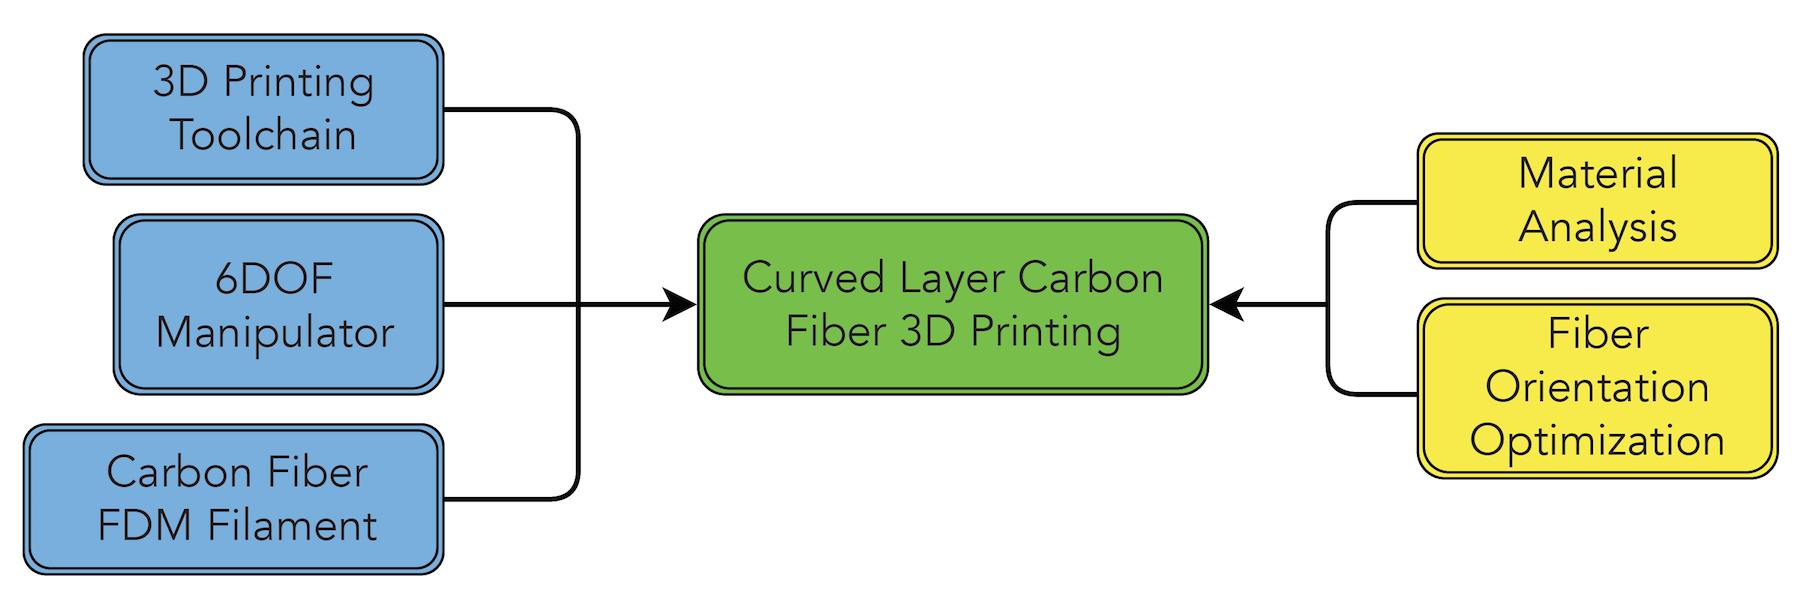
\includegraphics[width=1\textwidth]{./figures/flowchart}
\caption{A flow chart of subsystems.}
\label{fig:flowchart}
\end{figure}

%To realize the goal of a fiber-reinforced composite curved layer 3D printer, we will first learn to use to the FANUC LR Mate 200iC robot in The Cooper Union’s ME Rapid Prototyping Lab. This robot arm provides the necessary degrees of freedom for curved layer printing. We first plan to familiarize ourselves with the arm and control software by developing tool paths within its operational envelope. Then, we can mount an extruder to the arm and use an existing software toolchain to create standard flat-layer thermoplastic FDM prints. Once the standard print method is implemented, we can implement new gcode to create curved layer thermoplastic prints, while simultaneously investigating the best fiber composite to use as printing material. We will then alter the extruder mechanism to work with the chosen material. Finally, with curved layer fiber-reinforced 3D printing achieved, we plan to experimentally compare the mechanical strength of curved layer fiver-reinforced FDM prints to thermoplastic flat-layer FDM prints; the Instron machine in The Cooper Union’s ME Materials Lab can be used to load the parts and strain gauges can be attached to the parts to monitor specific local stresses.